\chapter{A quick travel in the history of crowdsourcing}
\label{chap:history-crowdsourcing}
\section{History of crowdsourcing}
\label{sec:history-of-crowdsourcing}
Crowdsourcing in its most general form is not new. We have records of large crowdsourcing experiments leading to high achievements in socio-economics fields and even playing parts in wars. Let us consider one historical example.

One of the eldest and most impactful happened in 1848 and is reported extensively in \citet{tracksinthesea}. Led by Matthew Fontaine Maury (an oceanographer between many other titles), the U.S. Naval Observatory distributed free copies of his book \emph{Wind and Current Charts} which described how to effectively reduce time travel at sea, see \Cref{fig:wind-current} -- \emph{shippers knew that every day saved at sea cut costs and lessened the danger of losing ships, cargoes and crews}. In return, Maury asked sailors to record standardized logs and return them to him at the U.S. Naval Observatory.
This form came with a ten-page instruction pamphlet on how to interpret the charts and how to fill out the logs.
The experiment ran for years, and even at the early beginning shipmasters wanted to increase their profit and participate: \emph{By September, the logs began flowing into the observatory, and Maury and his staff were busy trying to handle the volume}.
Collecting this information led to reducing the Rio de Janeiro - New York was then fifty-five days and was reduced to twenty-three in 1853.
They simplified and extended the charts with the full support of Navy captains and merchant companies like Forbes of Boston and Robert C. Wright of Baltimore for their sailors to fill out these forms.
More importantly, they noticed some sailors did not use the charts correctly, and this helped prove the importance of taking into account winds and currents at sea.
The newly collected data also helped create monthly recommendation charts for sailors.
\begin{figure}[ht]
    \centering
    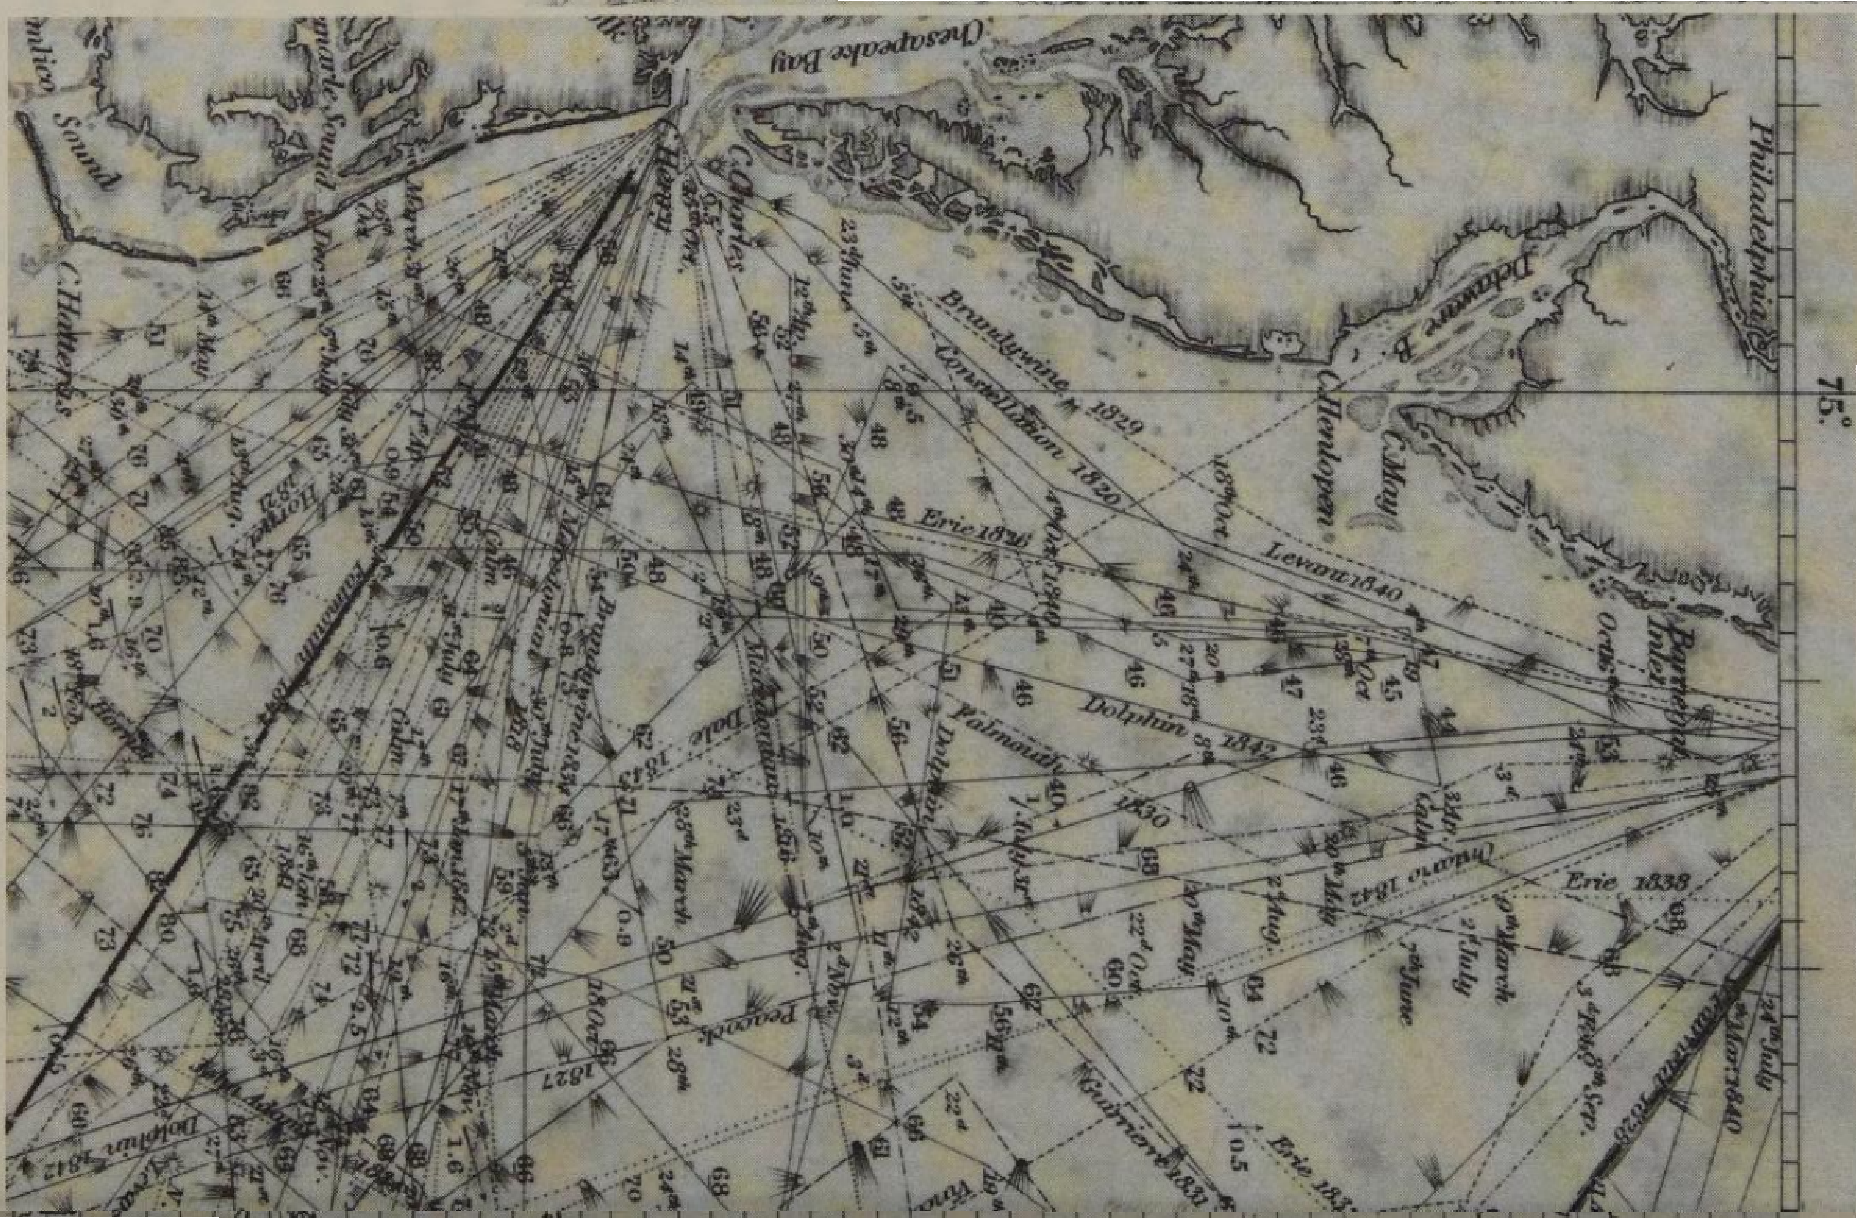
\includegraphics[width=.7\textwidth]{chapters/images/windmaps.pdf}
    \caption{Extract of the first edition of Wind and Current Chart of the North-Atlantic (1848) by Matthew Fontaine Maury. The brushes show the direction wind blows and their strength. The currents are shown with arrows. We can also see the water temperatures around the Chesapeake Bay.}
    \label{fig:wind-current}
\end{figure}

But the history of Maury's logs implications did not stop at currents and winds. In 1851, they released charts showing the distribution of sperm whales in oceans for each season -- an example is shown in \Cref{fig:whale-chart}. These tracks were used by whalers, but also during the Civil War by confederates to track Union ships that captured and harvested animals \footnote{\url{https://www.nytimes.com/1865/08/27/archives/the-pirate-shenandoah-her-cruise-in-the-arctic-seas-wholesale.html}}. This disrupted the North's economy as sperm whale's oil was popular for soaps, lubricants and also as light sources \footnote{\url{https://www.nytimes.com/2008/08/03/nyregion/03towns.html}}.
\begin{figure}[ht]
    \centering
    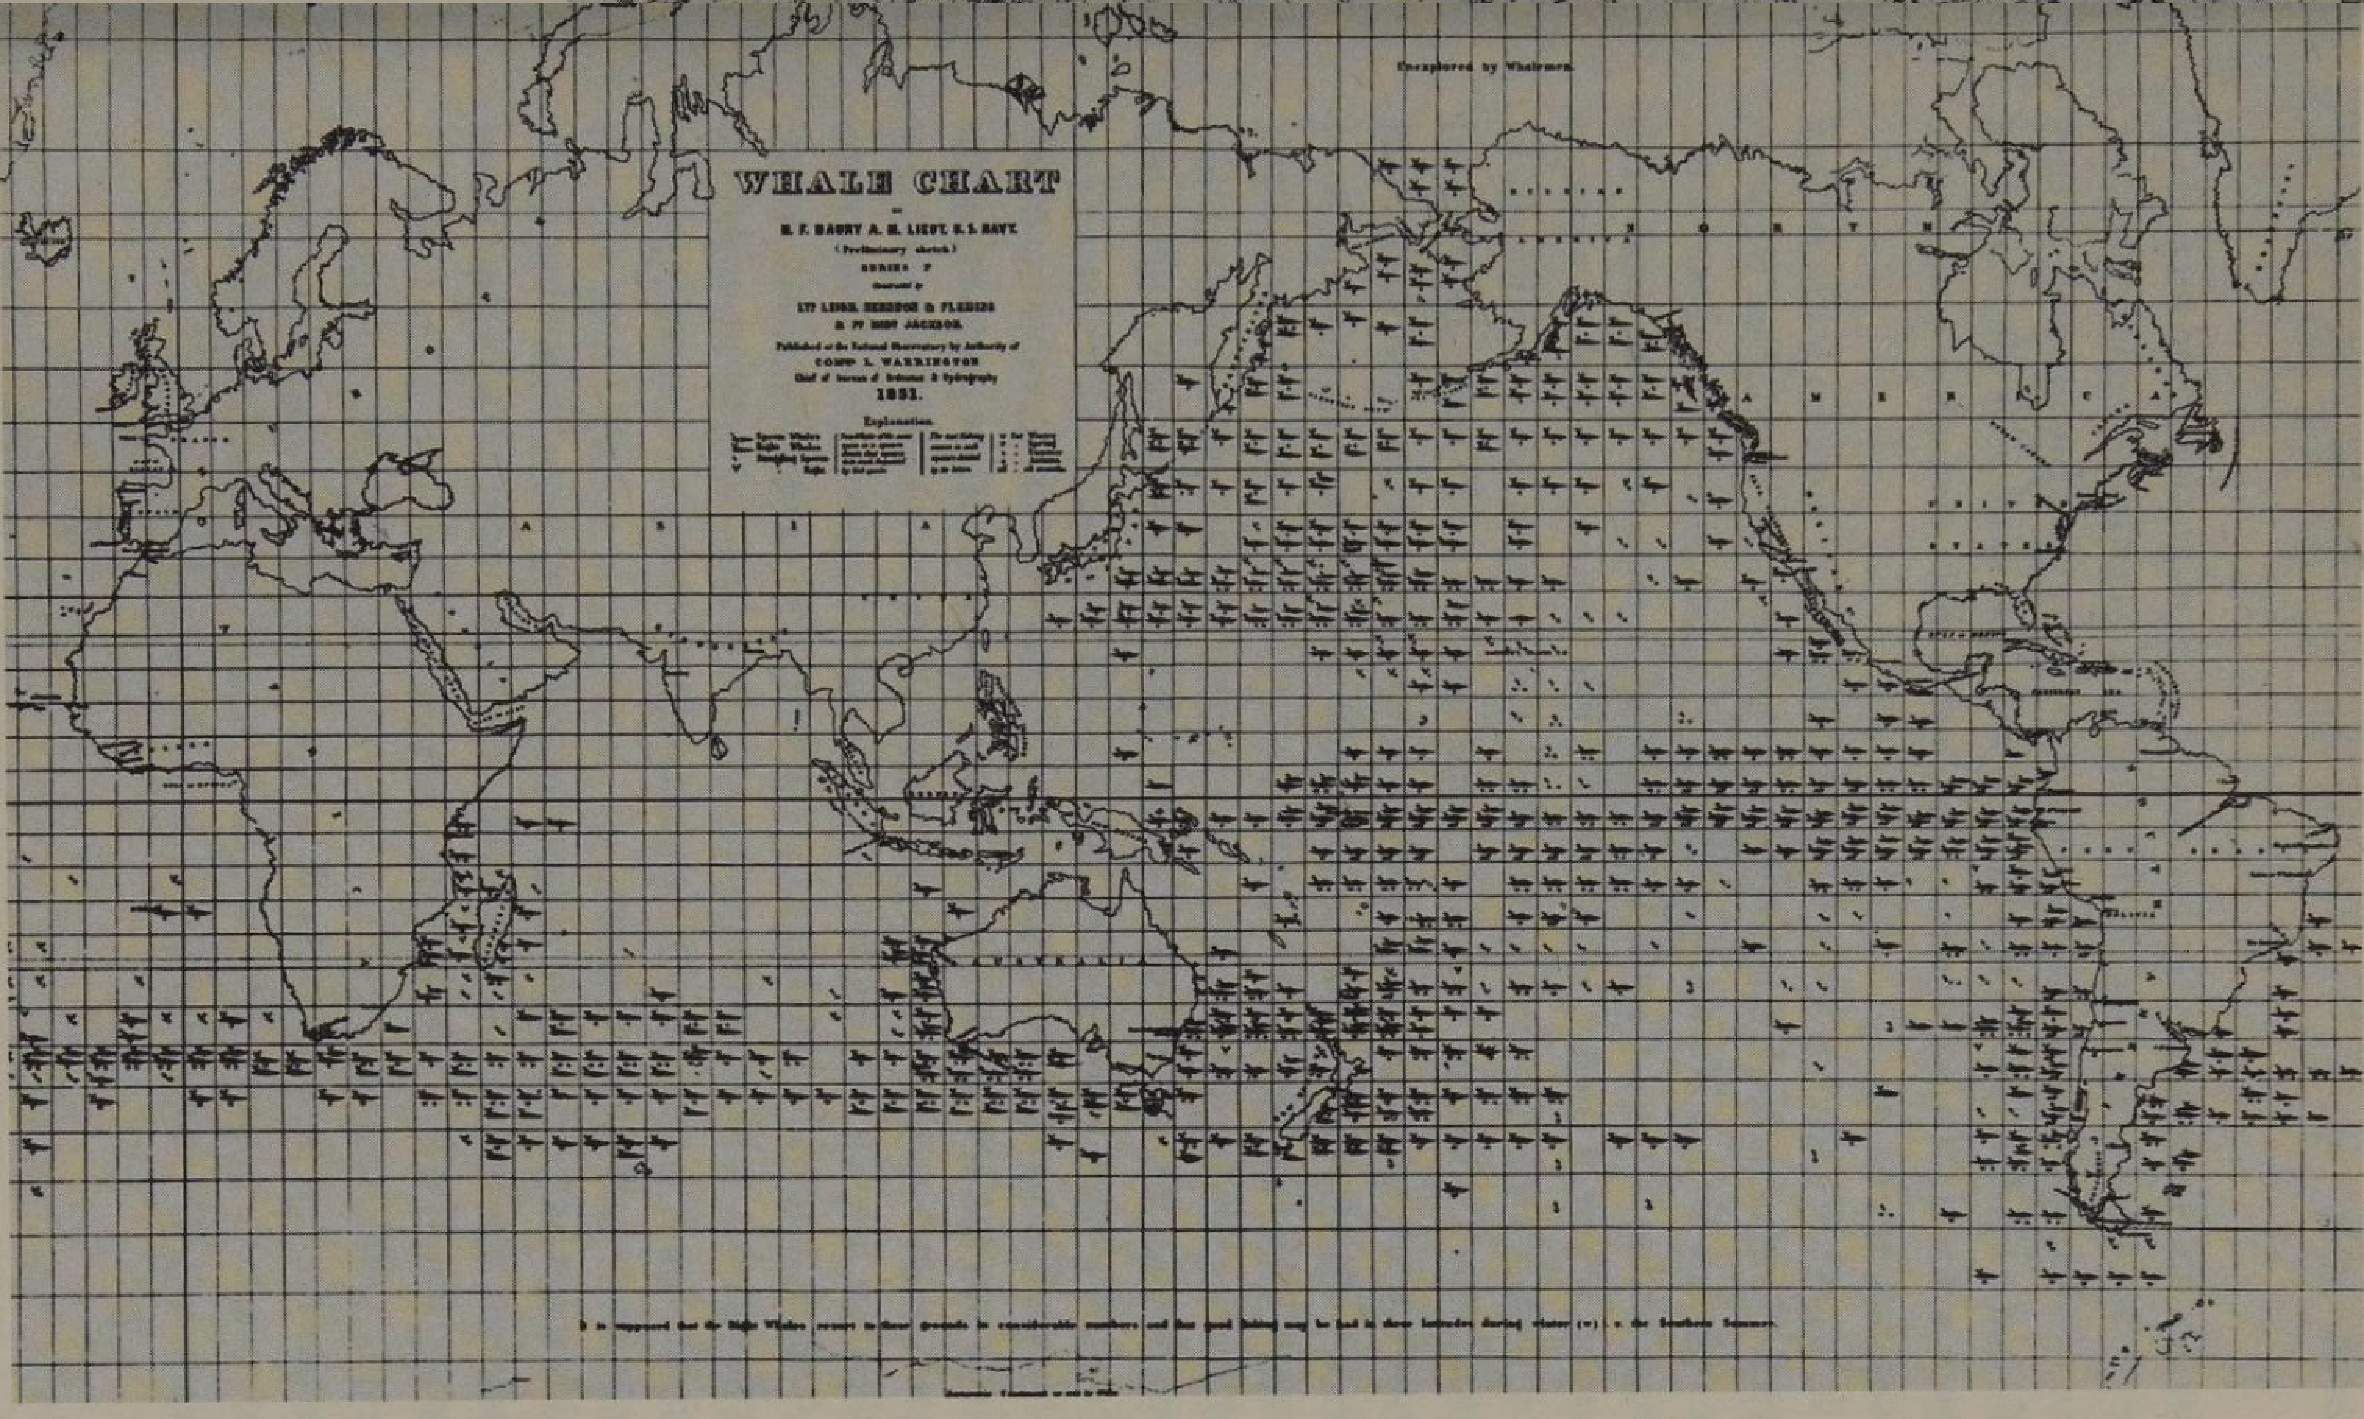
\includegraphics[width=.7\textwidth]{chapters/images/whales.pdf}
    \caption{Whale chart by Matthew Fontaine Maury from 1851, series F showing the distribution of sperm whales across oceans.}
    \label{fig:whale-chart}
\end{figure}

\section{Defining crowdsourcing}
\label{sub:definition-crowdsourcing}

Even though crowdsourcing isn't new, this is not the case for its proposed definition.
Because of its large possibilities of applications and the increasingly extensive use of the internet to conduct crowdsourcing experiments, there are multiple definitions of the term.

One of the first was recorded in 2006 by two journalists at Wired, Jeff Howe and Mark Robinson:
\begin{center}
\begin{minipage}{.75\textwidth}
    \emph{Simply defined, crowdsourcing represents the act of a company or institution taking a function once performed by employees and outsourcing it to an undefined (and generally large) network of people in the form of an open call. This can take the form of peer-production (when the job is performed collaboratively), but is also often undertaken by sole individuals. The crucial prerequisite is the use of the open call format and the large network of potential laborers.}
\end{minipage}
\end{center}
Later, Howe proposed to divide it into two definitions\footnote{\url{https://crowdsourcing.typepad.com/cs/2006/06/crowdsourcing_a.html}}:
\begin{center}
\begin{minipage}{.75\textwidth}
\begin{itemize}
    \item \emph{The White Paper Version: Crowdsourcing is the act of taking a job traditionally performed by a designated agent (usually an employee) and outsourcing it to an undefined, generally large group of people in the form of an open call.
}
    \item \emph{The Soundbyte Version: The application of Open Source principles to fields outside of software.
}
\end{itemize}
\end{minipage}
\end{center}

With the increasing use and misuse of the word crowdsourcing, \citet{estelles2012towards} provided a broader internet-based definition that was extracted from merging definitions from forty papers -- from a database of journal and conference papers about crowdsourcing containing 209 papers. The definition is as follows:
\begin{center}
\begin{minipage}{.75\textwidth}
\emph{
Crowdsourcing is a type of participative online activity in which an individual, an institution, a non-profit
organization, or company proposes to a group of individuals of varying knowledge, heterogeneity, and
number, via a flexible open call, the voluntary undertaking of a task. The undertaking of the task, of variable complexity and modularity, and in which the crowd should participate bringing their work, money, knowledge and/or experience, always entails mutual benefit. The user will receive the satisfaction of a given type of need, be it economic, social recognition, self-esteem, or the development of individual skills, while the crowdsourcer will obtain and utilize to their advantage that what the user has brought to the venture, whose form will depend on the type of activity undertaken.
}
\end{minipage}
\end{center}

One of their criteria was to explicitly take into account the "internet" factor to define modern crowdsourcing, thus this does not apply to experiments like Matthew Fontaine Maury's (\Cref{sec:history-of-crowdsourcing}). However, in the context of this thesis, and given how the vast majority of crowdsourcing experiments are nowadays used thanks to the internet, this definition is sufficient for our research purposes.

More importantly, the definition of crowdsourcing does not include peer production.
These two are often mixed up, but experts \citep{brabham2013crowdsourcing} differentiate them with multiple criteria -- the most important being the guidelines.
Let us take from \citet{brabham2013crowdsourcing} the example of one of the largest peer-production projects: Wikipedia.
It can not be considered a crowdsourcing project as there is no guideline given on what should be in an article or how it should be structured.
There is also no vertical control.
Wikipedia is controlled via peer assessments, so it is a horizontal control through dialogues.
In a crowdsourcing experiment, a crowdsourcer (company, laboratory,\dots) provides the task(s) and what should be done to complete them.
This can be as simple as \emph{Describe the image} or \emph{click on the bike}, or more complicated like \emph{can the second part of the proposition be inferred from the first part?} but the main point is that there is a clear guideline given directly to the worker to complete the task(s) at hand.

\section{Explicit and implicit crowdsourcing}
\label{sub:explicit-and-implicit}

From the multiple definitions of the term crowdsourcing, we see that broad implications lead to multi-faceted types of work.
More than the task itself to be completed, it is important to record how the tasks were presented to workers.
We know from \Cref{sub:definition-crowdsourcing} that a guideline plays a crucial part in the experiment.
However, a guideline can hide the purpose of an experiment. So crowdsourcing has been divided between two categories \citep{andro2017digital}:
\begin{itemize}
    \item implicit crowdsourcing: recourse to involuntary work by Internet users,
    \item explicit crowdsourcing: recourse to voluntary work from voluntary Internet users.
\end{itemize}

A famous example of implicit crowdsourcing tasks is the \texttt{reCAPTCHA} created by Luis von Ahn.
The principle is simple, we need to archive old books, and sometimes text recognition systems can not recognize the words -- for numerous reasons such that, and not exhaustive, paper quality, symbols and calligraphy, overlapping words -- and those words are given to write out to people on the internet just as ordinary security systems (see \Cref{fig:recaptcha}).
Most of the time, there are two \texttt{CAPTCHA}s to solve, one for control and then the actual task.
During the whole solving time, the worker does not know that they are solving an actual problem for a crowdsourcer, hence the implicit.
Multiple other examples for each are presented in \Cref{sub:run-experiments} with a more detailed classification of crowdsourcing tasks.

\begin{figure}[ht]
    \centering
    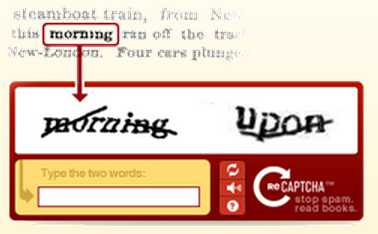
\includegraphics[width=.5\textwidth]{chapters/images/recaptcha.jpg}
    \caption{Example of \texttt{reCAPTCHA} from 2014 for word recognition tasks. The word here is \texttt{morning} and the control word \texttt{upon}.}
    \label{fig:recaptcha}
\end{figure}


\section{Current ways to classify and run experiments}
\label{sub:run-experiments}

Defining types of crowdsourcing is not the same as defining types of crowds.
In \citet{kazai2011worker} created five worker profiles: spammer, sloppy, incompetent, competent, and diligent. In \citet{martineau2012typology} workers are classified as communal, lurkers, utilizers and aspirers.
This quest for worker profile identification is still an active field of research.

But taking a step back in this problem, \citet{brabham2013crowdsourcing} proposes a typology to classify crowdsourcing experiments: not tasks nor workers.
\begin{itemize}
    \item knowledge discovery and management: find and collect standardized information -- \emph{e.g} Flag association application to register discrimination and act of violence against LGBTQ+ people for the French government\footnote{\url{https://www.flagasso.com/}},
    \item broadcast search: solve empirical problems -- \emph{e.g} coding challenges as Kaggle
    \item peer-vetted creative production: create and select creatives ideas -- \emph{e.g} Threadless\footnote{\url{https://www.threadless.com/}} allow its community to create designs for shirts or prints and then puts them to a vote each week,
    \item Distributed-human-intelligence tasking; analyze large amounts of information -- \emph{e.g} label images or part of images like Pl@ntNet.
\end{itemize}

In practice, running a crowdsourcing experiment has been eased up by platforms such as Amazon Mechanical Turk\footnote{\url{https://mkturk.com/}} or Toloka\footnote{\url{https://toloka.yandex.com}}.
These marketplaces allow to conduct of a paid experiment -- ethical considerations apart (and discussed in \cref{sub:ethics}) -- that is planned with extensive parametrization.
The data labeling is outsourced so you don't need to think about the resource allocations. They also have algorithms (some like \citet{raykar_ranking_2011} that we discuss in \Cref{chap:peerannot}) to detect unreliable workers to have better data.

\begin{figure}[ht]
        \centering
        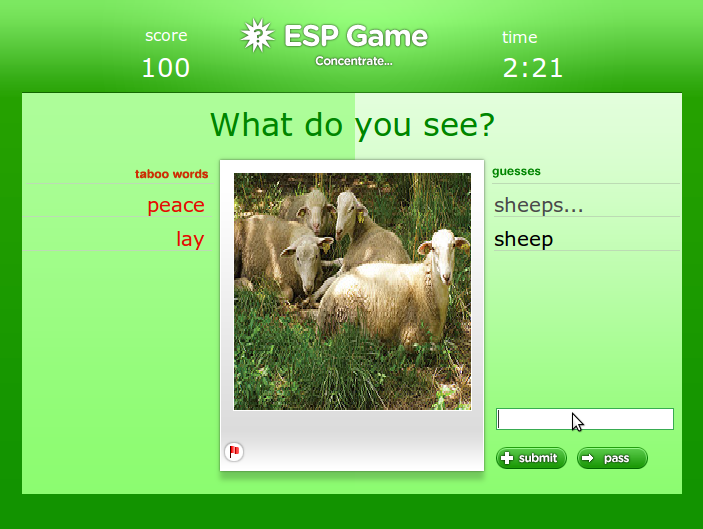
\includegraphics[width=.6\textwidth]{chapters/images/ESP.png}
        \caption{Example of ESP game image (from \url{https://edutechwiki.unige.ch}). The image represents four sheep laying in the grass. The first worker proposes \texttt{sheep} and then \texttt{sheep} at the second round. Note that to avoid having the same labels by multiple workers for the images, taboo words were introduced. In this case, workers were forbidden to answer the words \texttt{peace} and \texttt{lay} to describe the image. Not every image had taboo words.}
        \label{fig:ESP-game}
\end{figure}

However, paying workers is not the only way to collect crowdsourced data.
The gamification of crowdsourcing tasks has proved to be quite efficient with experiments like Eyewire \citep{tinati2017investigation}, ThePlantGame \citep{plantgame2016}, \emph{etc}.
Luis Von Ahn (the \texttt{CAPTCHA} creator) was one of the first researchers on GWAPs (Games With A Purpose).
He famously also founded in 2004 the ESP (ExtraSensory Perception) game \citep{von2005esp} to create metadata on images --  presented in \Cref{fig:ESP-game}.
Two players are paired up randomly and shown the same image.
They can not communicate, but they each can provide a single word to describe the image presented.
Once they both provide the same word, the game stops.
They have 2 minutes and 30 seconds to label 15 images.
At one point, they can both choose to pass on a single image.
A license was bought by Google to create the Google Image Labeler\footnote{\url{http://news.bbc.co.uk/2/hi/technology/7395751.stm}} from 2006 to 2011.

We have seen paid workers and playing workers, but sometimes workers just participate voluntarily without any second motivation from the crowdsourcer.
This is the case in Pl@ntNet where the workers' only gain in participating is providing more data to improve the model's prediction for the community. Here, the gain is scientific and the participation is based on providing better tools for the community -- a sense of having participated to help others.
RTE, France also created a crowdsourcing platform\footnote{\url{https://www.bdpv.fr/_BDapPV/}} to identify photovoltaic panels on images and delimit their area of occupancy \citep{kasmi2023crowdsourced}.

In short, with crowdsourcing, we can classify workers, types of tasks/experimentation and the incentives to make workers answer those tasks. Each of these parts can play a role in the data collection process and quality of said data.

\chapter{Peerannot appendix}
\label{chap:app-peerannot}

\section{Code structure to implement the DS model}
\label{app:DS}

In \texttt{peerannot}, iterative label aggregation strategies need a \texttt{.run()} method. We present an example of such a structure with the DS model in \Cref{listing:DS}.


\section{Simulated mistakes with discrete difficulty levels on tasks}
\label{sec:difficulty-levels}
For an additional experiment, we consider the so-called discrete difficulty setting presented in \citet{whitehill_whose_2009}. Contrary to other simulations, we here consider that workers belong to two levels of abilities: \texttt{good} or \texttt{bad} and tasks have two levels of difficulties: \texttt{easy} or \texttt{hard}. The keyword \texttt{ratio-diff} indicates the prevalence of each level of difficulty of tasks as:
\[\texttt{ratio-diff} = \frac{\mathbb{P}(\texttt{easy})}{\mathbb{P}(\texttt{hard})}, \text{ with }\mathbb{P}(\texttt{easy}) + \mathbb{P}(\texttt{hard})=1 \enspace.\]

Tasks that are \texttt{easy} are answered correctly by every assigned worker. Tasks that are \texttt{hard} are answered following the confusion matrix assigned to each worker. Each worker then answers independently to the presented tasks.

We simulate $200$ tasks and $100$ workers with $35\%$ of good workers and $50\%$ of \texttt{easy} tasks (\texttt{ratio-diff}$=1$). There are $K=5$ classes. Each task receives $|\mathcal{A}(x_i)|=10$ votes.
\begin{listing}[ht]
    \begin{minted}[linenos=true, bgcolor=lightgray, tabsize=4, fontfamily=courier, fontsize=\small, xleftmargin=5pt, xrightmargin=5pt]{bash}
$ peerannot simulate --n-worker=100 --n-task=200 \
                     --n-classes=5 \
                     --strategy discrete-difficulty \
                     --ratio 0.35 \
                     --ratio-diff 1 \
                     --feedback 10 \
                     --seed 0 \
                     --folder ./simus/discrete_difficulty
    \end{minted}
    \caption{Simulation of discrete difficulty levels crowdsourced datasets in \texttt{peerannot}.}
\label{listing:discrete_simu}
\end{listing}

\begin{table}[htbp]
    \centering
    \caption{AccTrain metric on simulated mistakes made when tasks are associated with a difficulty level considering classical feature-blind label aggregation strategies.}
    \label{tab:accuracy_train_diff}
    \begin{tabular}{|l|c|c|c|c|c|c|}
    \hline
    \textbf{Strategy} & \textbf{MV} & \textbf{GLAD} & \textbf{DS} & \textbf{DSWC[L=2]} & \textbf{DSWC[L=5]} & \textbf{NS} \\
    \hline
    AccTrain & 0.815 &	0.845 &	0.810 &	0.600 &	0.660 &	0.790 \\
    \hline
    \end{tabular}
    \end{table}

Finally, in this setting involving task difficulty coefficients, the only strategy that involves a latent variable for the task difficulty, knowing GLAD, outperforms the other strategies (see \Cref{tab:accuracy_train_diff}). Note that in this case, creating clusters of answers leads to worse decisions than an MV aggregation.

\begin{figure}[htbp]
    \centering
    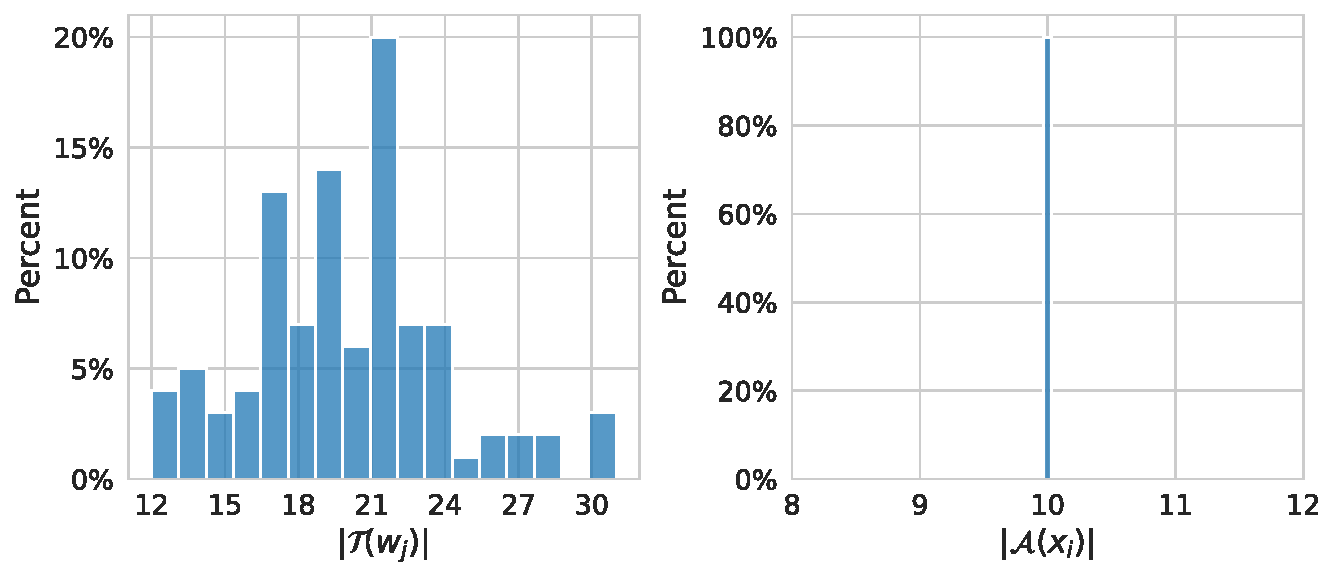
\includegraphics[width=.8\textwidth]{./chapters/images_peerannot/cell-20-output-1.pdf}
    \caption{Distribution of the number of tasks given per worker (left) and of the number of labels per task (right) in the setting with simulated discrete difficulty levels.}
\end{figure}

\begin{listing}[ht]
    \begin{minted}[linenos=true, bgcolor=lightgray, tabsize=4, fontfamily=courier, fontsize=\small, xleftmargin=5pt, xrightmargin=5pt]{python}
class Dawid_Skene(CrowdModel):
    def __init__(self, answers, n_classes, **kwargs):
        super().__init__(answers)
        ...

    def get_crowd_matrix(self):
        ... # Convert json answers to tensor (task, worker, label)

    def init_T(self):
        ... # Initialize the confusion matrices

    def m_step(self):
        """Maximizing log likelihood
        Returns:
            p: (p_j)_j class marginals
            pi: confusion matrices
        """
        ...

    def e_step(self):
        """Estimate indicator variables
        Returns:
            T: New estimate for the labels (n_task, n_worker)
        """
        ...

    def log_likelihood(self):
        ... # Compute the log likelihood of the model

    def run(self, epsilon=1e-6, maxiter=50):
        self.get_crowd_matrix()
        self.init_T()
        k, eps, ll = 0, np.inf, []
        while k < maxiter and eps > epsilon:
            self.m_step()
            self.e_step()
            likeli = self.log_likelihood()
            ll.append(likeli)
            if len(ll) >= 2:
                eps = np.abs(ll[-1] - ll[-2])
            k += 1

    def get_probas(self):
        return self.T

    def get_answers(self):
        return np.vectorize(self.converter.inv_labels.get)(
            np.argmax(self.get_probas(), axis=1)
        )
\end{minted}
\caption{MWE for the DS label aggregation in \texttt{peerannot}.}
\label{listing:DS}
\end{listing}

\clearpage

\chapter{Table of strategies used}
\label{sec:tab-strategies}
Here, we provide a table resuming the strategies used in the experiments presented in this thesis and some of their specificities.

% \begin{longtable}[htbp]
    \begin{center}
    \begin{longtable}{|l|p{15mm}|p{35mm}|p{25mm}|p{40mm}|}
        % \caption{Table of strategies used in the experiments presented in this thesis.}
        % \label{tab:strategies}
    \hline
    \textbf{Strategy} & \textbf{Type} & \textbf{Full name} &  \textbf{Paper} & \textbf{In short}\\
    \hline
    MV & aggregate & Majority vote & -- & -- \\
    NS & aggregate & Naive soft & -- & Frequency of votes \\
    DS & aggregate & Dawid and Skene's & \citet{dawid_maximum_1979} & Model worker with confusion matrix \\
    WDS & aggregate & Weighted with Dawid and Skene's & -- & Use DS diagonal to represent worker abilities \\
    Fast-DS & aggregate & Fast Dawid and Skene's & \citet{sinha2018fast} & DS aggregate with Dirac representation of the estimated labels \\
    GLAD & aggregate & Generative models of Labels, Abilities and Difficulties & \citet{whitehill_whose_2009}& Models task difficulty and worker ability as scalar values  \\
    DSWC & aggregate & Dawid and Skene's with Worker clustering & \citet{imamura2018analysis} & Clustered DS model over the workers\\
    WAWA & aggregate & Worker Agreement With Aggregate & Appen & Worker ability is the accuracy against MV labels \\
    MACE & aggregate & Multi-Annotator Competence Estimation & \citet{hovy2013learning} & Worker ability is the accuracy against MV labels \\
    KOS & aggregate & Karger, Oh and Shah & \citet{karger2011iterative} & Binary classification using graph representation \\
    TwoThird & aggregate & -- & -- & Label with at least two votes and a two-third of consensus is accepted \\
    \hline \hline
    CrowdLayer & inference & -- & \citet{rodrigues2018deep} & Confusion matrices as a new layer in the neural network \\
    CoNAL & inference & Common Noise Adaptation Layers & \citet{chu2021learning} & Local confusion and shared confusion as new layers\\
    \hline \hline
    AUM & identify (task) & Area Under the Margin & \citet{pleiss_identifying_2020} & Identify ambiguous tasks in classical supervised setting\\
    AUMC & identify (task)& Area Under the Margin for crowdsourcing & \citet{lefort2022improve} & Identify ambiguous tasks with MV aggregation \\
    WAUM & identify (task)& Weighted Area Under the Margin & \citet{lefort2022improve} & Identify ambiguous tasks relative to worker abilities \\
    Entropy & identify (task) & -- & -- & Identify worker abilities with entropy of NS labels\\
    Spam Score & identify (worker) & -- & \citet{raykar_ranking_2011} & Identify spammers via DS matrices\\
    Trace confusion & identify (worker) & -- & -- & Identify poor workers via DS matrices' trace\\
    Krippendorff's $\alpha$ & identify (dataset) & -- & \citet{krippendorff1980validity} & Identify unreliable crowdsourced datasets\\
    \hline
    \end{longtable}
\end{center}
%     \end{tabular}
% \end{table}
